\documentclass[11pt, oneside]{article} 
\usepackage{geometry}
\geometry{letterpaper} 
\usepackage{graphicx}
	
\usepackage{amssymb}
\usepackage{amsmath}
\usepackage{parskip}
\usepackage{color}
\usepackage{hyperref}

\graphicspath{{/Users/telliott_admin/Tex/png/}}
% \begin{center} 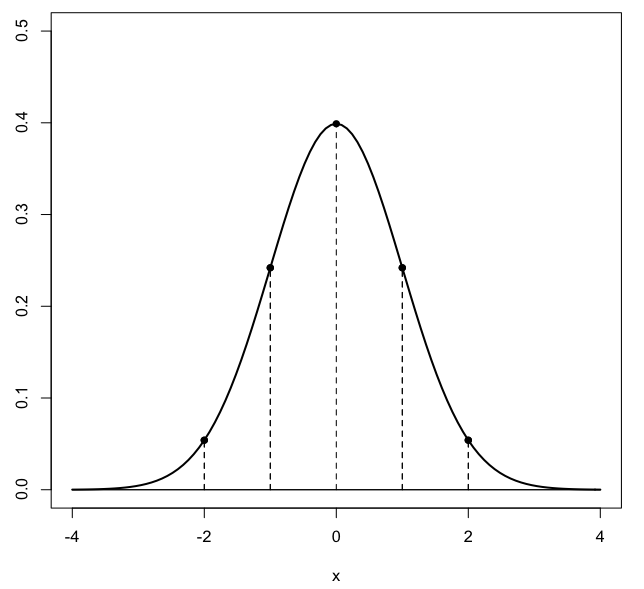
\includegraphics [scale=0.4] {gauss3.png} \end{center}

\title{Calculus in Five Minutes}
\date{}

\begin{document}
\maketitle
\Large

\label{sec:Calc_Five}

The essential ideas of calculus are surprisingly simple. See if you don't agree.

We talk about the slope of a curve at a single point. This seems odd because "slope" refers to a change in $y$ divided by a change in $x$. We ought to need two points, not just one. But we don't.

A single point can have a slope for the same reason that the earth seems to be flat where I'm standing right now even though I know it is really curved---it is flat, on the ocean or a desert highway at least.

The carpenters who built your house assumed that the earth's curvature is negligible, and we will too. We can mentally zoom in indefinitely (ask an ant if the earth is flat).

\begin{center} 
\includegraphics [scale=0.4] {Calc5_1.png} \end{center}

So for any given point on a curve, we can always find another point very close nearby which has the same slope, and then we know the slope between them is constant (within any limits you want to establish).

\begin{center} 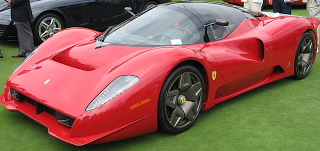
\includegraphics [scale=0.4] {Calc5_2.png} \end{center}

\subsection*{Like driving a car}

You can understand the basic procedures in calculus by thinking about driving a car. Most drivers refer frequently to the speedometer (which measures velocity), while if they want to know about distance they use the odometer. 

If we plot accumulated distance as a function of time, the slope of that curve is the velocity shown on the speedometer. [This analogy will become useful in a bit].

There are tricks to use to find the slope from the equation for a curve. Where the tricks come from isn't hard to understand, but it's not necessary---just use the trick. Consider the equation:

\[ (y-1) = (x-2)^2 \]
Multiply it out to make things a bit more interesting:
\[ y = x^2 - 4x + 5 \]

The trick is that the slope of this curve (designated as y') is easily calculated:
\[ y' = 2x - 4 \]

We used three rules: 

(i) if we have various parts being added together, we take the slope for each part separately and then add them up.

(ii) the slope of a constant term (like $y = 3$) is zero (obviously, a horizontal line is flat, and has slope equal to 0).

(iii) lastly, the formula for powers of $x$.  If
\[ y  = c x^n \]
($c$ stands for constant);  then
\[ y' = c n x^{n-1} \]

\subsection*{So what}
One reason this is useful is to find maximum and minimum points of a curve. These are points at which the slope is zero. For our example

\[ y' = 2x - 4 = 0 \]
\[ x = 2 \]
This happens when
\[ y = x^2 - 4x + 5 = 4 - 8 + 5 = 1 \]

This is easy to see by going back to the first form of the equation. Because of the square, the minimum occurs when the term in parentheses on the right is zero.
\[ (y-1) = (x-2)^2 \]

There are other simple tricks for terms like $e^x$ and $\sin x$.

I mentioned that a car's odometer and speedometer perform related tasks, and these are a good way to think about the fundamental operations of calculus. Suppose a car is going in a straight line (say, on the freeway across the Nevada desert). We need to deal only with the positive $x$-axis. 

Distance (often labeled $s$) is a function of time:
\[ s = f(t) \]

If the velocity is constant and we start from s = 0 then:
\[ s = v \times t \]

Distance equals velocity times time. Travel at $60$ miles per hour for $2$ hours and you'll go $120$ miles.

On the other hand, velocity might be changing with time. Let's say we'll figure out how it changes later, and just write in a general way:
\[ v = f(t) \]

If the velocity is changing, we call the rate of change in velocity the acceleration. (It is the slope of the curve for $v$ as a function of $t$). If the acceleration is constant (like gravity), then:
\[ v = a \times t \]

For a car, imagine increasing the pressure on the gas pedal steadily so that after $1$ second you are going $10$ mph, after $2$ seconds $20$ mph, after $3$ seconds $30$ mph. If we continue at the same rate, we'll accelerate from $0$ to $60$ mph in $6$ seconds.

What it is depends on the exact form of $s$ as a function of time. If the acceleration is constant:

\[ s = \frac{1}{2} a t^2 \]

Remember the rule from above?
\[ y  = c x^n \]
\[ y' = n c x^{n-1} \]

Or, using the time and distance symbols:
\[ s  =  \frac{1}{2} a t^2 \]
\[ s' = v = a t \]
\[ s'' = a \]

So that is where the factor of $1/2$ comes from in the equation involving acceleration. It is needed to cancel the the $2$ that comes out of the exponent when we differentiate. One way to think about this is to say that the velocity after a period of constant acceleration is the average of the initial acceleration and the final acceleration, times the time. But this differentiation mumbo jumbo will work even if the velocity and acceleration are more complicated functions of time.

Differentiation is useful, but integration allows us to do things which are nothing short of miraculous. For example, consider this modestly complex equation, and its curve.
\[ y = x^3 - x^2 - x + 150 \]

\begin{center} 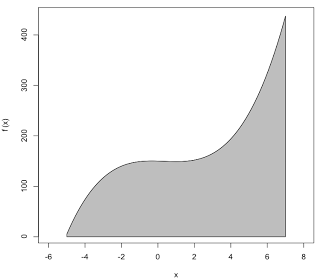
\includegraphics [scale=0.6] {Calc5_3.png} \end{center}

\subsection*{integration}

The integral calculus allows us to easily calculate the area under this curve and above the $x$-axis, as shown in gray.

Remember what we said before: the relationship between the function which we plot as a curve, and its slope at any point is found by differentiating $f(x)$ to $f'(x)$. The slope is $f'(x)$. 

The secret of integral calculus (don't tell anybody) is that the same relationship holds between the area under a curve, and the curve itself, but in reverse. That is, if the curve is $f'(x)$, the area is $f(x)$. It's that simple.

If we know $f'(x)$, how do we find $f(x)$? Sometimes it's easy and sometimes it's hard. Suppose that every time we have a function $f(x)$ and we find $f'(x)$, we write the result down and save it in our little black book. When we encounter a function in an integration problem, we look in the book.

For the example, we need a function $f(x)$, which when differentiated gives:

\[ y' = x3 - x2 - x + 150 \]

We look in our book, and there it is:
\[ y = \frac{1}{4}x^4 - \frac{1}{3} x^3 - \frac{1}{2} x^2 + 150 x \]

Of course, the area depends on which endpoints we choose. (Looking at the figure should make this clear). So evaluate the integrated function between the limits x = 7 and x = -5. We have:

\[ 74/4 - 73/3 - 72/2 + 7*150 \]
minus
\[ (-5)4/4 - (-5)3/3 - (-5)2/2 + (-5)*150 \]

I get:
\[ 2401/4 - 343/3 - 49/2 + 1050 - 625/4 + 125/3 - 25/2 - 750 \]
The rest is just arithmetic.

I'm too lazy to finish it. But I'll check the method itself by an interesting approach later.

Why do I say it's a miracle? Because we get the area from the integrated equation just by using the endpoints. We don't have to worry about what lies between. That is amazing.


\end{document}